%% This is emulateapj reformatting of the AASTEX sample document
%%
\documentclass{emulateapj}
\usepackage{amsmath}

%% You can insert a short comment on the title page using the command below.

%\slugcomment{Report for Independent Research}

%% If you wish, you may supply running head information, although
%% this information may be modified by the editorial offices.
%% The left head contains a list of authors,
%% usually a maximum of three (otherwise use et al.).  The right
%% head is a modified title of up to roughly 44 characters.
%% Running heads will not print in the manuscript style.

\shorttitle{Determination of Kinematic Inclinations}
\shortauthors{Beauchemin}

%% This is the end of the preamble.  Indicate the beginning of the
%% paper itself with \begin{document}.

\begin{document}

%% LaTeX will automatically break titles if they run longer than
%% one line. However, you may use \\ to force a line break if
%% you desire.

\title{Determining Galaxy Inclinations from Kinematics}


%% Use \author, \affil, and the \and command to format
%% author and affiliation information.
%% Note that \email has replaced the old \authoremail command
%% from AASTeX v4.0. You can use \email to mark an email address
%% anywhere in the paper, not just in the front matter.
%% As in the title, use \\ to force line breaks.

\author{Ryan Beauchemin, Charlie Bonfield, Kirsten Hall, Sheila Kannappan}
\affil{Department of Physics and Astronomy, University of North Carolina at Chapel Hill}
%\email{rwbeauchemin@unc.edu}

%\author{Names of second author -- delete if not relevant}
%\affil{Astronomy Department, University of Florida, Gainesville, FL 32611}

%\and

%\author{Name of Third author -- delete if not relevant}
%\affil{Space Telescope Science Institute, Baltimore, MD 21218}


%% Mark off your abstract in the ``abstract'' environment. In the manuscript
%% style, abstract will output a Received/Accepted line after the
%% title and affiliation information. No date will appear since the author
%% does not have this information. The dates will be filled in by the
%% editorial office after submission.

\vspace{1cm}\begin{abstract}
%The distribution of inclinations of spiral galaxies in any area in the sky is expected to be completely random in an isotropic universe. Surprisingly, we find that this is not the case when using inclinations determined from the projected shape of the galaxy or photometric inclinations. 
\large We compare photometric inclinations with kinematic inclinations, derived from the distribution of Doppler shifted velocities for galaxies of the RESOLVE survey, using data taken by the 4.1m SOAR telescope and Goodman spectrograph. To measure the velocities, we determine the kinematic inclinations first using the publicly available DiskFit routine, which takes a number of points in discrete elliptical annuli and fits based on the radial averages of velocities within those annuli. Finding problems in the output of DiskFit for galaxies that are poorly-sampled, we develop a code that uses all data points simultaneously: Velocity Field Fitter (VFF). We intend to implement this code in the same manner, but we first quantify the differences between the two fitting methods by testing how they fare when high turbulence is added to an artificial velocity field or when the amount of velocity field points is low. This is done in order to determine the success of their application as turbulence and sampling are varied. 
\end{abstract}

%---------------------------------------------------------------------------------%
%                             Section 1: Introduction                             %
%---------------------------------------------------------------------------------%

\section{Introduction}

\large The distribution of spiral galaxies in any area in the sky is expected to be completely random in an isotropic universe. It is fairly common in a luminosity-limited survey to purport any deviation from randomness to the fact that smaller or more edge-on galaxies give off less light. However, in our volume-limited REsolved Spectroscopy Of a Local VolumE (RESOLVE) galaxy survey it is found that the distribution of observed axial ratios expected when randomly looking this is not the case when using inclinations determined from the projected shape of a galaxy, or photometric inclinations. In this section, I motivate why photometric inclinations could be inaccurate, why kinematic inclinations are needed, and why the RESOLVE survey helps us to understand the differences.

\subsection{Photometric Inclination}

\large Inclinations are defined as the projected tilt of a disk galaxy ranging from 0 to 90 degrees, or from face-on to edge-on. We have analyzed galaxies of the RESOLVE catalog photometrically using the axial ratio of the projected ellipse to determine its inclination by the classic formula from \citet{hubble}

\begin{equation}
i = cos^{-1}(((q^2-q_0^2)/(1-q_0^2))^{1/2})
\end{equation}

\noindent \large where $q$ is the major to minor axial ratio and $q_0$ is the ratio at an inclination of 90 degrees. Since disk galaxies are not flat, $q_0$ must be greater than 0, and is taken to be 0.2, as determined by \citet{holmberg}. The axial ratios for this equation are found using SDSS data and the IRAF ``ellipse'' task to map an ellipse to the outer isophotes of our galaxies.

%\begin{figure}
%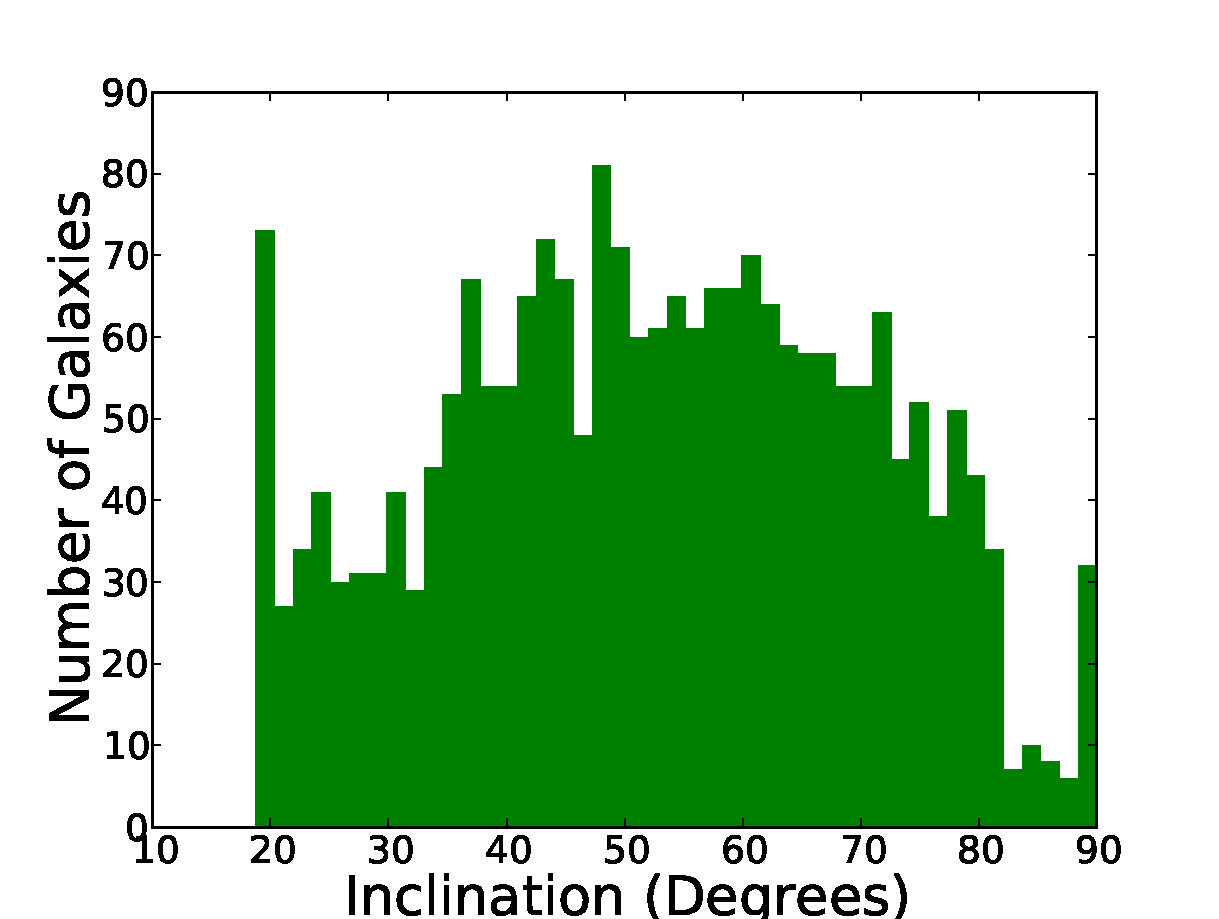
\includegraphics[width=0.5\textwidth]{hist1.pdf}
%\caption{The distribution of photometric inclinations in the RESOLVE survey. If the measurement was truly random, this distribution should be fairly flat. \label{fig:test}}
%\end{figure}

\large We are interested in finding why this is the case, as we would expect there to be no preference in a volume-limited survey. The root of this problem may lie in either the way that photometric inclinations are calculated or in our understanding of the intrinsic shapes of disk galaxies. I have been working towards ruling out one of these options in answering the question: Is our current method of photometric inclination determination sound, and if not, what photometric properties cause this error? This is an important question to tackle because, for almost a century, galactic astronomers have been using an equation that assumes a lot about the shape and structure of a galaxy but has not yet been tested vigorously for robustness. Luckily, there is another way to determine the inclination of galaxies that assumes much less about the structure, using its kinematics.

\subsection{Kinematic Inclination}

\large Kinematic inclinations are inclinations found from the observed velocity fields of spiral galaxies. These galaxies rotate about a central point and their line-of-sight velocities from Doppler shifting can be detected by a spectrograph to determine the average velocities of baryonic matter in the line of sight. Using the velocity field data with the maximum velocity calculated from luminosity as described by \citet{tullyfish}, one may determine how far a galaxy is from edge-on. This can be done because an observed edge-on galaxy would have almost all of its velocity in the line of sight. In contrast, a face-on galaxy would show only the cosmological redshift at most of the points in the galaxy. One may model the distribution of possible inclinations based on the velocity fields. This can be seen in the equation relating projected velocities with inherent velocities described by \citet{teuben}
\begin{equation}
\large V(x,y) = V_{sys}+V_{rot}(R)\cos{\theta}\sin{i}
\end{equation}

\noindent \large where $\theta$ is the angle of the deprojected galaxy, and $i$ is the inclination from (1). We believe that the kinematic method of inclination measurement is more accurate because, by probing a third dimension, it makes less assumptions about the intrinsic properties of a spiral galaxy. Processes exist with the ability to tidally disturb velocities in some regions of galaxies, but the effects appear to be minimal when determining the inclination on a larger scale. With two different ways of measuring inclination, we have made a comparison of measurements using the two methods and how their differences relate to other properties of galaxies in order to see from where these differences arise. With the belief that the kinematic method provides a more accurate representation of a galaxy's true inclination, this also means that we might expose faults in the measurement of photometric inclinations.

\subsection{The RESOLVE Survey}
\large In the UNC-led RESOLVE, all galaxies in a nearby volume are observed regardless of size or luminosity. RESOLVE is considered to be volume-limited: Galaxies are selected between two redshifts and in a smaller, more resolved area in the sky. This type of survey is much more statistically representative of the composition of our universe than the classical approach which is limited by apparent brightness. In the latter approach, one obtains data for only the brightest galaxies. Such galaxies are not as common in the universe as dwarf or irregular galaxies. Though these surveys give us a good idea about the large scale structure of the universe, it is also pertinent to our understanding of the universe that we explore the details of the small-scale structure that makes up the large-scale structure. The RESOLVE team members at UNC are well-situated to observe local environments because UNC, as a partner, is guaranteed a portion of time every year and competes nationally for more time on the 4.1 meter SOAR telescope, located in Chile. The SOAR telescope is capable of taking highly-resolved (0.22 arc seconds per pixel) spectra of galaxies, and has an Atmospheric Dispersion Corrector (ADC). With the large number of observed galaxies in the RESOLVE survey, we can look at the distribution of photometric properties such as axial ratio, morphology, baryonic mass, and more with the expectation that most of them should be random in a volume-limited sample.
%---------------------------------------------------------------------------------%
%                                  Section 2: Data                                %
%---------------------------------------------------------------------------------%

\begin{figure}
%\plotone{rf0071example.pdf}
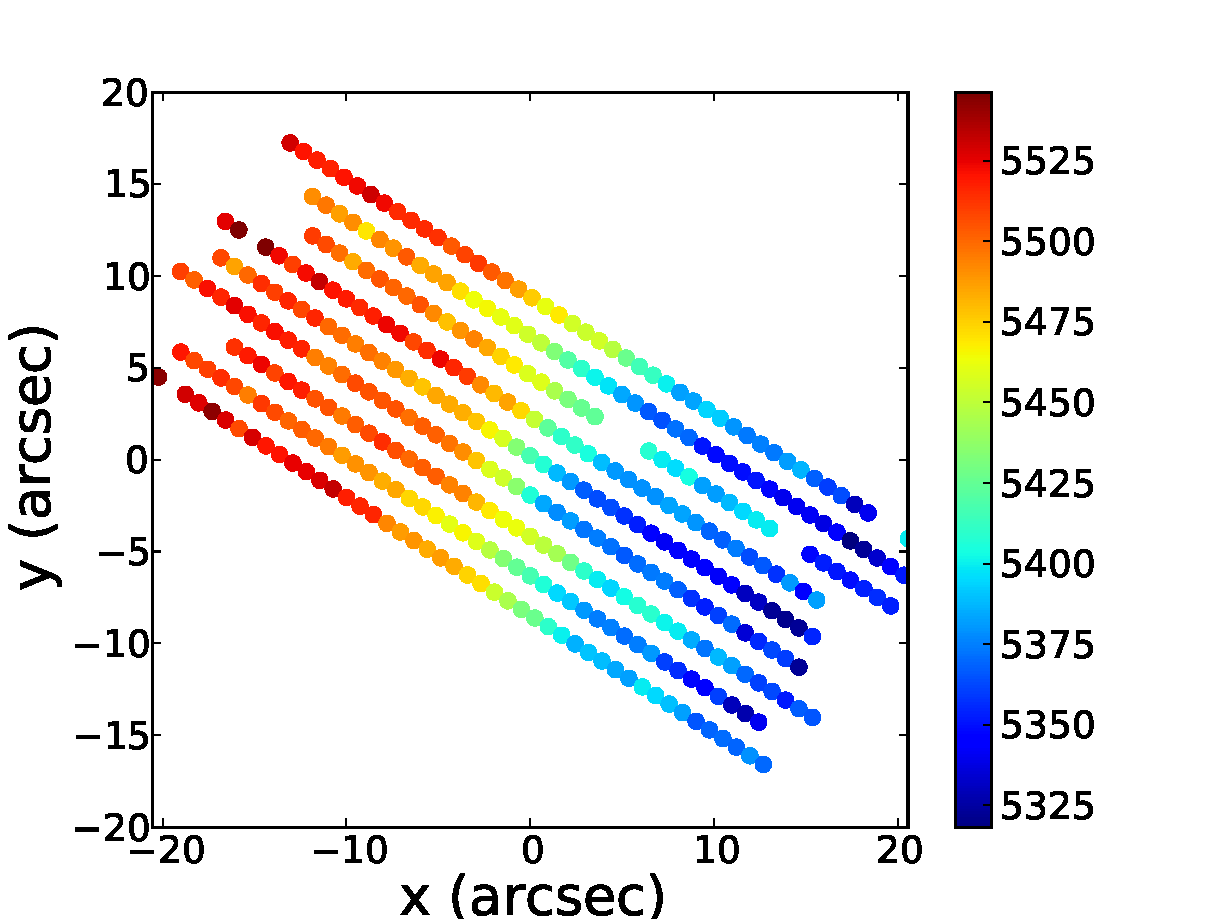
\includegraphics[width=0.5\textwidth]{rf0071example.pdf}
\caption{An example of the velocity field of a nearly face-on galaxy with three pointings from the fall catalog of the RESOLVE survey, with velocities given in km/s. \label{fig:test}}
\end{figure}


\section{Data and Sample}

\begin{figure}
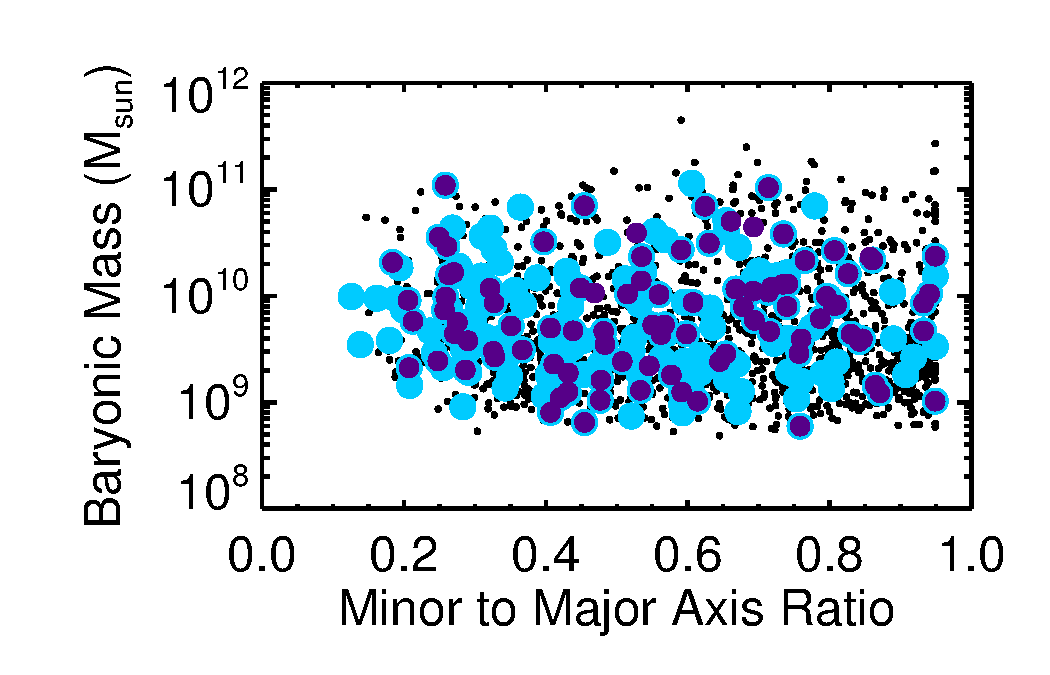
\includegraphics[width=0.5\textwidth]{naxisratio-eps-converted-to.pdf}
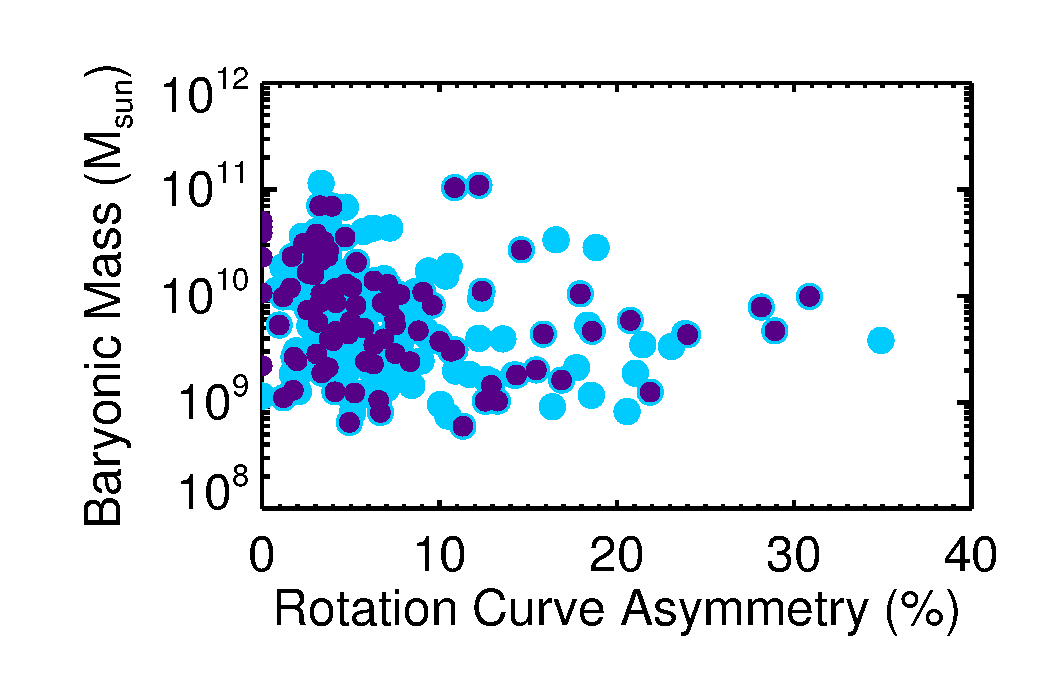
\includegraphics[width=0.5\textwidth]{nasymHa-eps-converted-to.pdf}
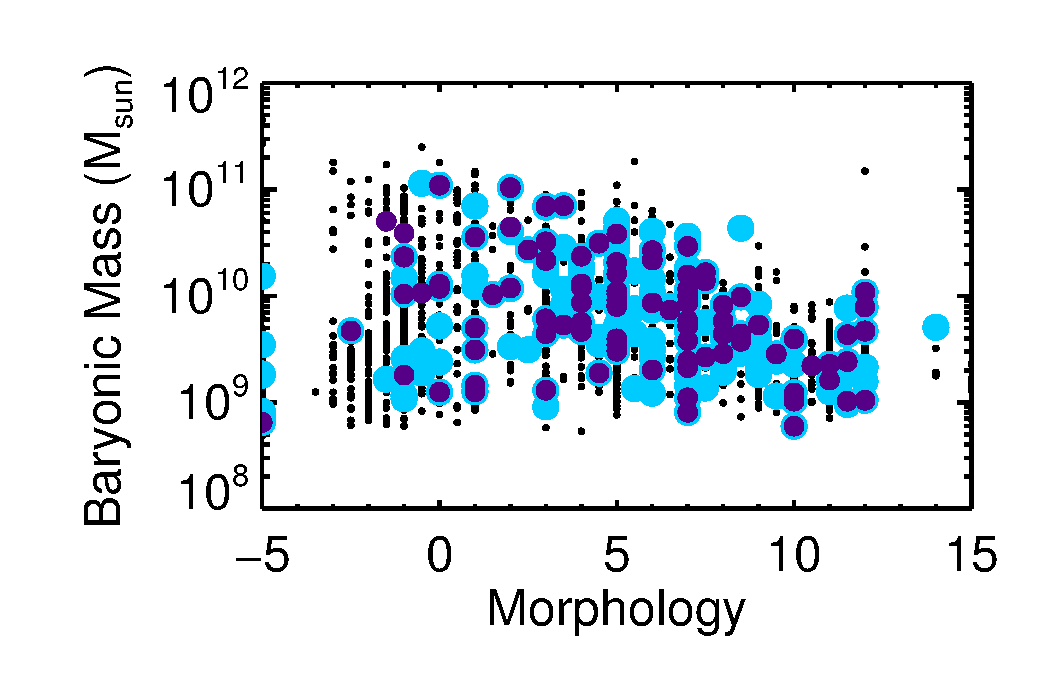
\includegraphics[width=0.5\textwidth]{nmorph-eps-converted-to.pdf}
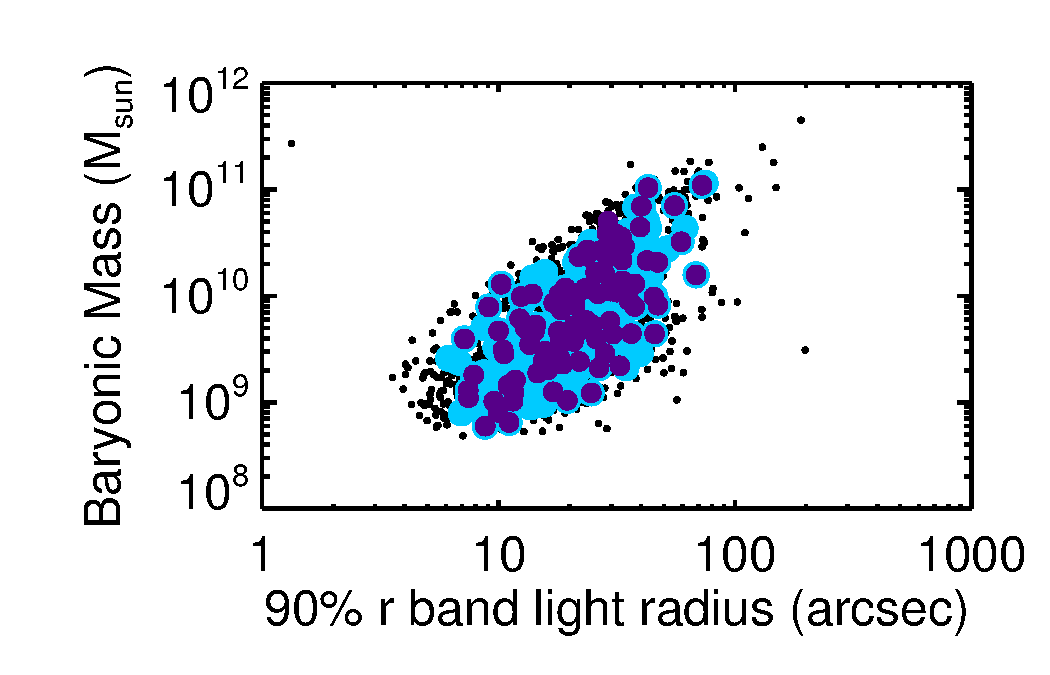
\includegraphics[width=0.5\textwidth]{nradr90p-eps-converted-to.pdf}

\includegraphics[width=0.5\textwidth]{stuff-Recovered-eps-converted-to.pdf}
\caption{Baryonic mass against axial ratio, rotation curve asymmetry, morphology, and 90\% r band light radius. \label{fig:test}}
\end{figure}

\large We observe galaxies using the 4.1m SOAR telescope and collect spectra using its GOODMAN spectrograph with a custom-built spectrograph image slicer that allows up to three nearby spectra to be taken at once without overlap. All data is reduced through a pipeline created by the RESOLVE team. Of the galaxies in the survey, a subsample including all previously reduced data was selected for the comparison of photometric and kinematic inclinations. To ensure that the sample was representative of the larger survey, we checked various properties of interest based on what we would expect might have an effect on the two dimensional projection of a galaxy or on the observed velocity field. This would in turn affect the photometric and kinematic inclination measurements respectively. Properties determined to have an effect are the galaxy's morphology, rotation curve asymmetry, and radius within which 90 percent of the galaxy's r-band light is contained. For statistical reasons, we also made sure to have a representative distribution of all the axial ratios found within the survey. This sample, when thoroughly examined, contains many very interesting phenomena: There is one galaxy with a hole punched through it, many galaxies that only have one slit of data from being edge-on, more that have rotating satellites, and a few face-on galaxies where one can see the random motions of baryonic matter above and below the plane of the disk. Since we need at least two slits of data to determine a kinematic inclination, we cannot quantify much about most edge-on galaxies, but we hope to be able to determine the inclinations of these other unique cases with our new fitting methods.


%---------------------------------------------------------------------------------%
%                           Section 3: Kinematic Vfitting                         %
%---------------------------------------------------------------------------------%

\section{Fitting Methods}

\subsection{DiskFit}

\large A publicly available code called DiskFit \citep{barnes} is capable of fitting the velocity field data that we have to a model profile given initial guesses to the position angle and galaxy center. Using DiskFit to model velocity fields for $\sim$100 galaxies, we have found there to be no clear link between the differences in photometric and kinematic inclination measurements and their respective galaxy properties such as total baryonic mass, rotation curve asymmetry, 90\% r-band radii, or morphology, but we did find some problems fitting small, asymmetric, or barred structures in the disk-fitting algorithm. This makes sense because the model requires many points in order to fit at many annuli and the program assumes the rotation curve to be inherently smooth, but perturbations might easily be misinterpreted, especially with the weight they would have in a small annulus.

\subsection{Velocity Field Fitting}

\large To remedy this, we have created a new algorithm that uses all of the data simultaneously, without having to fit disk annuli to it. We first find the center of kinematic rotation in the Doppler velocity field, then we use equations from \citet{teuben} that provide a translation from projected velocities to rotational velocities. Next, we map out the rotation curve of the galaxy and fit the rotation curve to the arctan function described by \citet{courteau}
\begin{equation}
\large v(r) = V_{0}+\frac{2}{\pi}v_{c}\arctan{R}
\end{equation}

\noindent \large and using chi squared minimization techniques described by \citet{mpfit} in Python. We have found that there is a distinct advantage in doing this for small galaxies that do not have enough data in each annulus to make a clear disk but still have enough information to give a reasonable kinematic profile. We have found also that kinematic inclinations are more random than their photometric counterparts, but we still have not compared the differences with other photometric properties, as we did before with the DiskFit models.

%%%%% MAKE THAT COMPARISON?? %%%%%%

%---------------------------------------------------------------------------------%
%                                Section 4: Results                               %
%---------------------------------------------------------------------------------%

\section{Results}
\large We employed various tests on VFF to see whether it holds up well to different problems in fitting velocity fields. Many of these tests involve first making a perfect velocity field, one which is generated to kinematically match the photometrically determined properties of a galaxy, and then introducing defects, finally examining the ability for the code to recognize properties of the original profile.

\subsection{Perfect Fields}
\large As a zeroth order test, we made sure that the re-examination of a perfect field (example shown in Figure 3) gave exactly the right inclination, and the correlation was a perfect one-to-one for well-sampled fields with no turbulence or other large perturbations in the field. DiskFit performed just as well in this test, which leads us to believe that both methods do very well for well-sampled galaxies.

\begin{figure}[h]
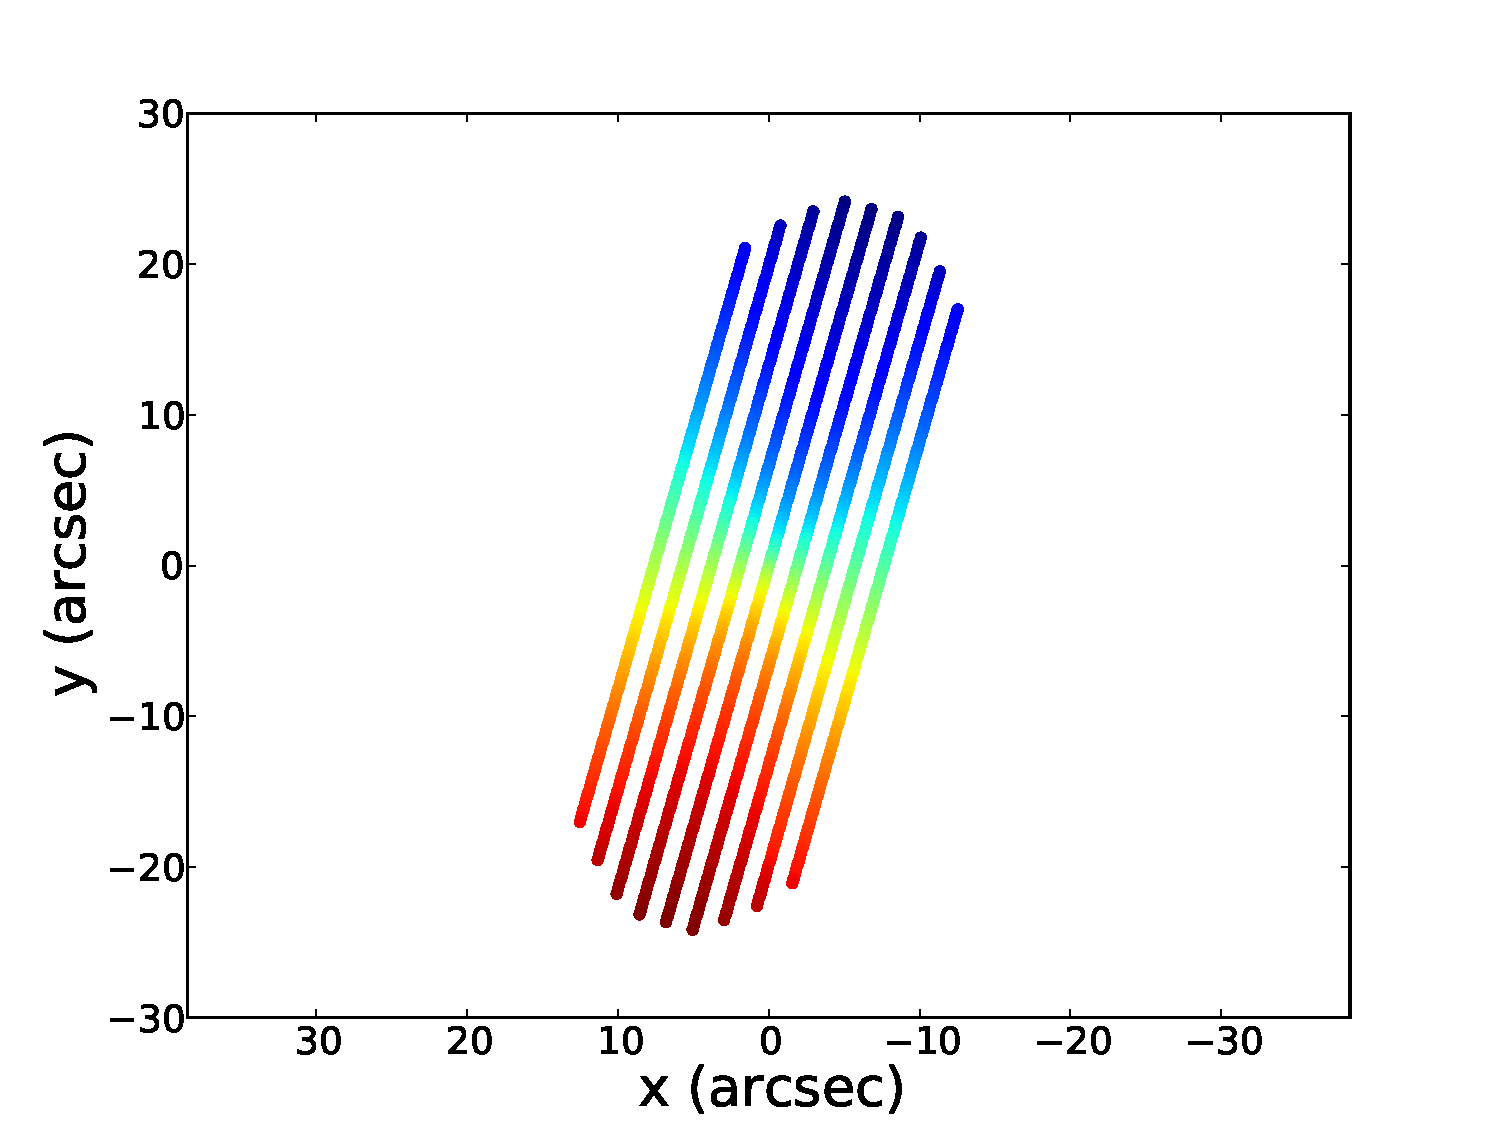
\includegraphics[width=0.5\textwidth]{perfectexamp.pdf}
\caption{An example of a velocity field generated by VFF to kinematically match the photometrically determined properties of a galaxy in the sample with three pointings with three slits in each. \label{fig:test}}
\end{figure}

\subsection{Fields with Turbulence}
\large Next, we introduced random Gaussian noise across the perfect velocity field to model turbulence. The re-examination for 60, 120, and 200 km/s yielded a one-to-one correlation with the original dataset. The example with turbulence is shown in Figure 4, and the results are in Figure 5. 
%%%%%HOW DOES VFF PERFORM VS DISKFIT? PLOT IT
%%%%%%% MAKE CHANGES HERE %%%%%%%%


\begin{figure}[h]
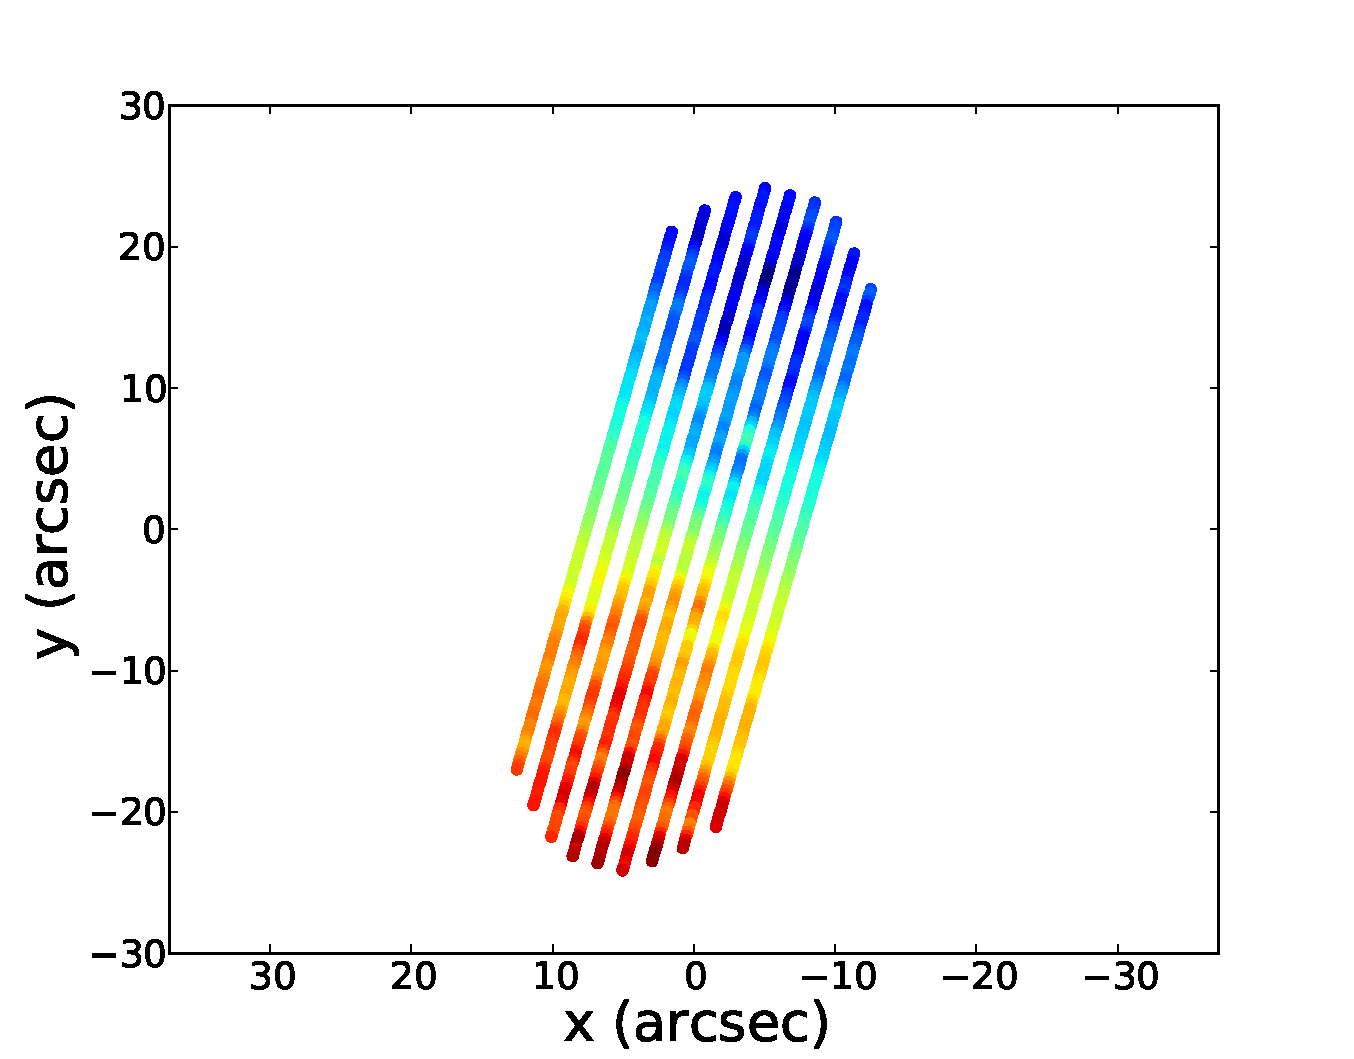
\includegraphics[width=0.5\textwidth]{turbexamp.pdf}
\caption{The same field from Figure 4, but with 120 km/s Gaussian noise added to the velocity. This models the effects of dust and atmosphere missed by the ADC.  \label{fig:test}}
\end{figure}

\begin{figure}[h]
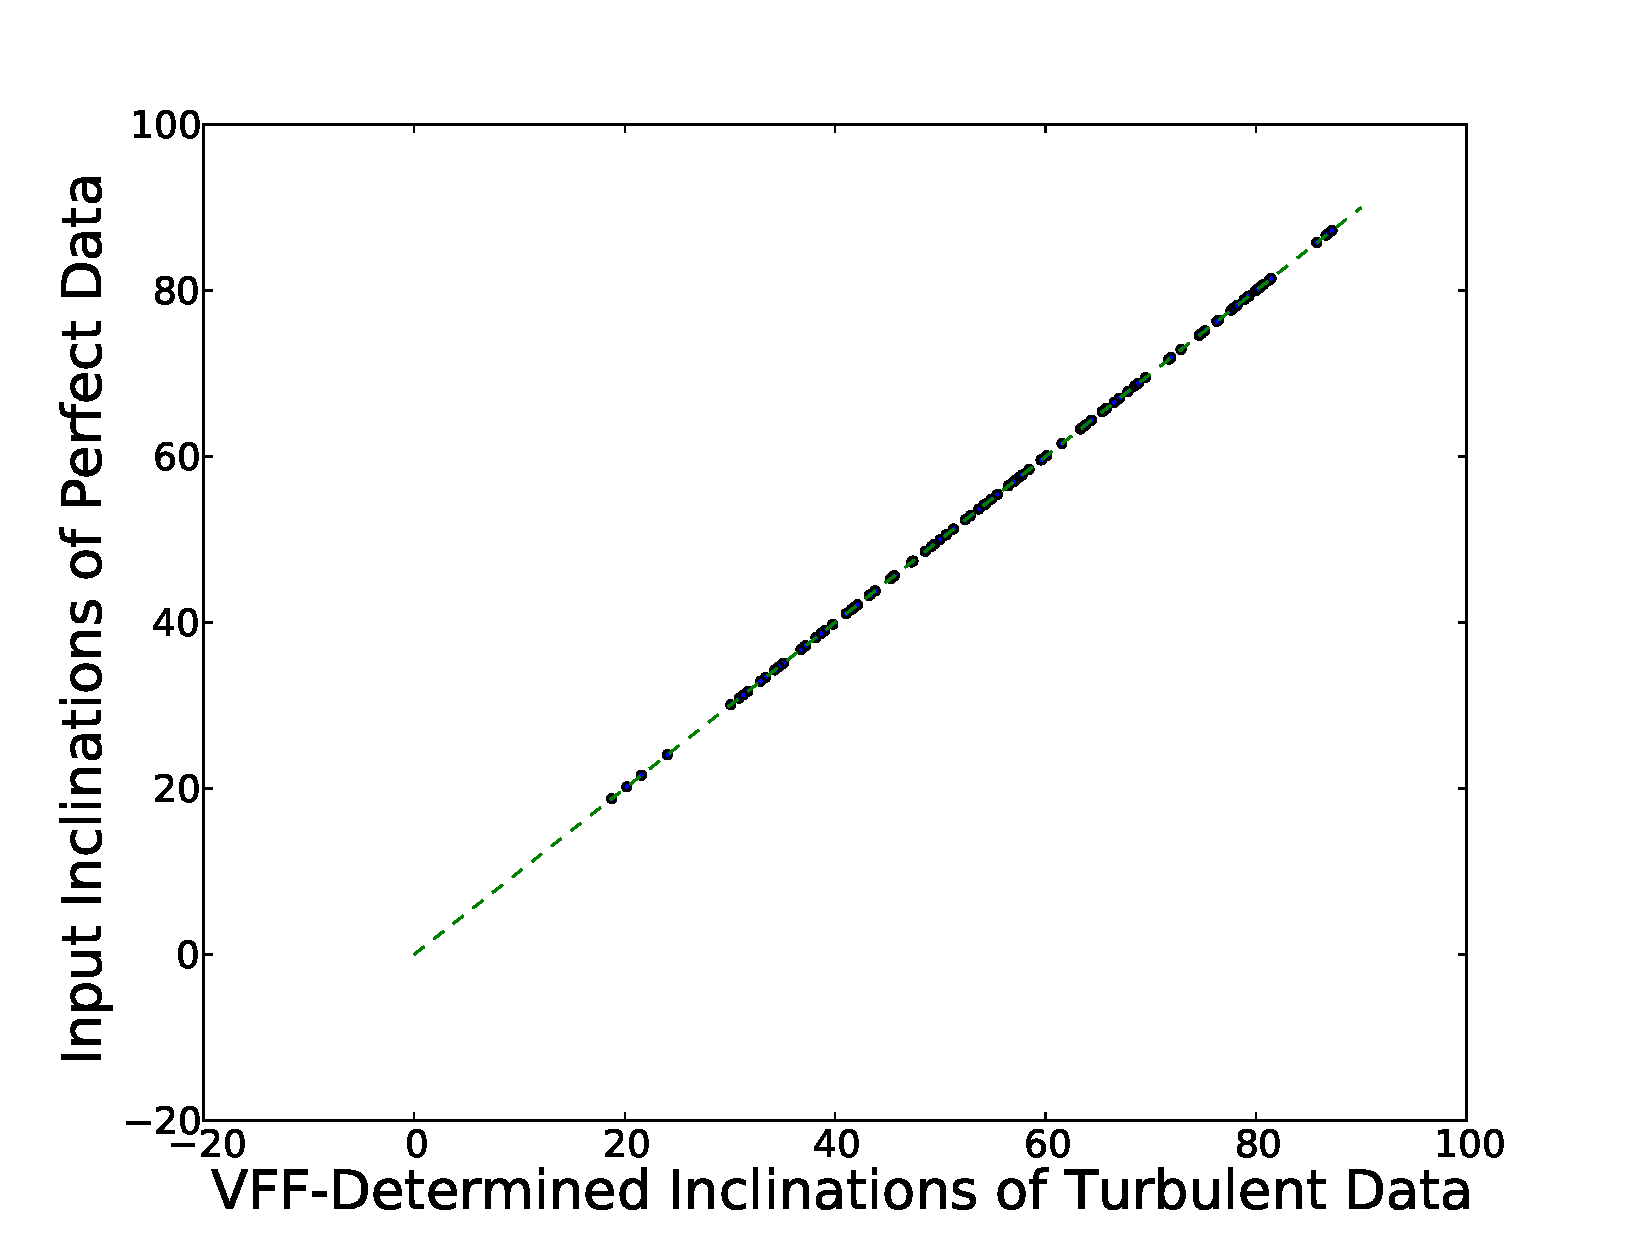
\includegraphics[width=0.5\textwidth]{turbtest.pdf}
\caption{The one-to-one correlation with input parameters and output parameters from VFF after 60 km/s turbulence was added. \label{fig:test}}
\end{figure}

\subsection{Binned Down Perfect Fields}
\large This test attempted to determine how the fitting process holds up against binned down data from the perfect fields to simulate the resolution of a realistic observation of a galaxy. In fact, for each galaxy we binned at the locations of the actual data from the RESOLVE survey, and used the distance between it and its nearest neighbor as the binning radius. This test gave DiskFit a lot of trouble, making half of the galaxies fail the Fortran fitting procedure that it employs (BRENT). VFF fit all of the galaxies that this test included, but it did not give a one-to-one correlation to the original properties, and fit on average to a lower inclination than the input. This effect is still being investigated in regards to a possible problem with longslit data, but it is promising that the routine does not give up so easily as DiskFit.

%%%%%% WRITE FINDINGS FROM CHECKING THIS!!! %%%%%%%%%

\begin{figure}[h]
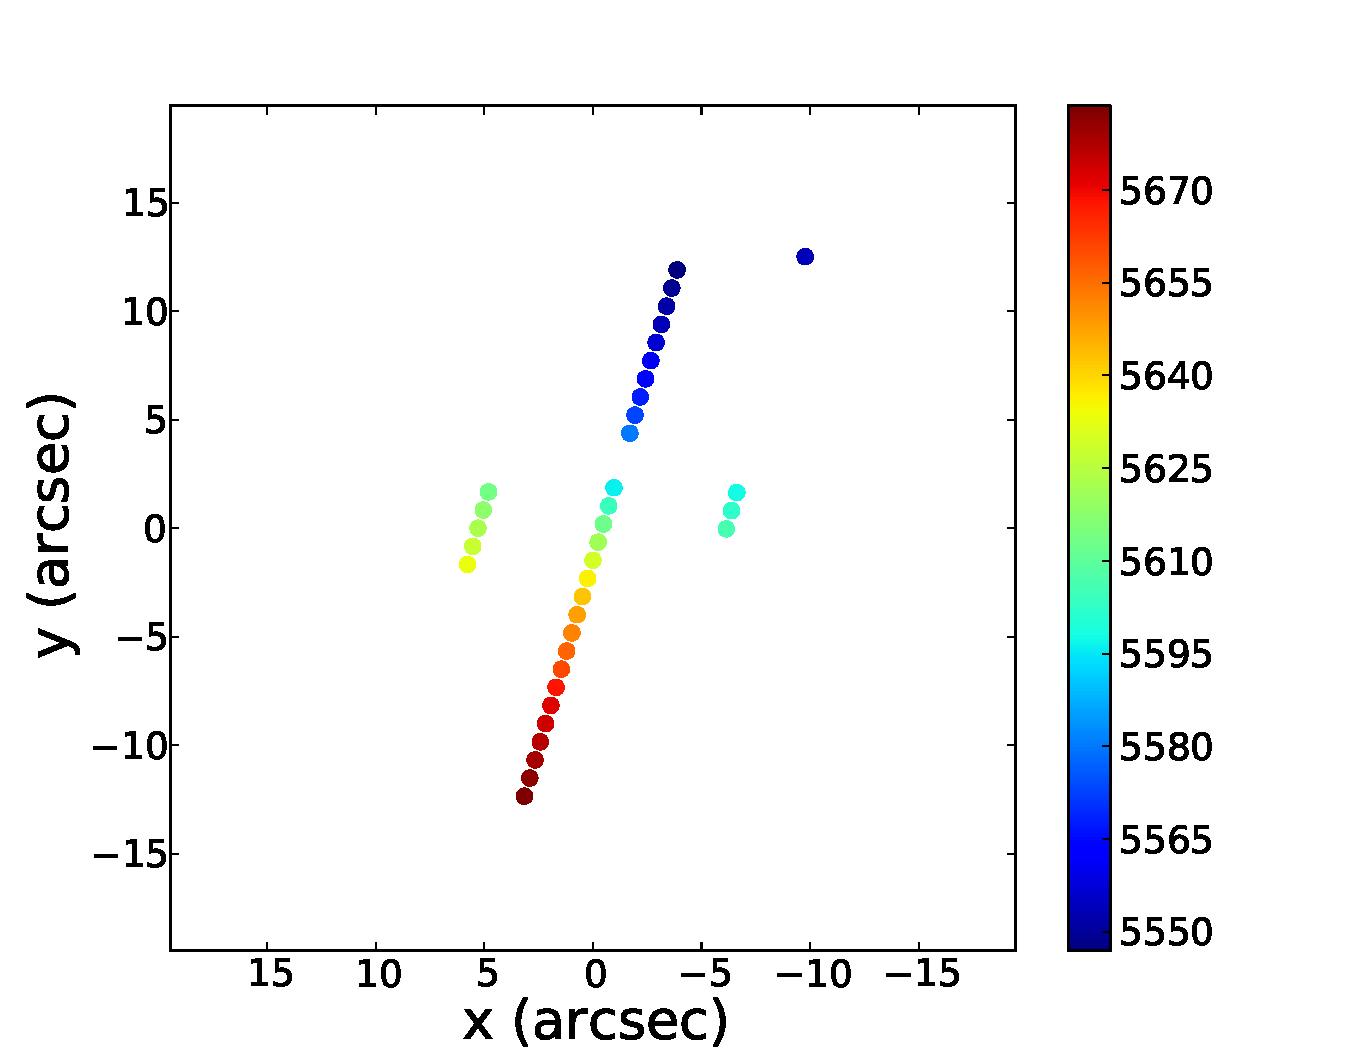
\includegraphics[width=0.5\textwidth]{binnedvels.pdf}
\caption{The field from Figure 4 with velocities binned to the resolution of the SOAR telescope for direct comparison. \label{fig:test}}
\end{figure}

\begin{figure}[h]
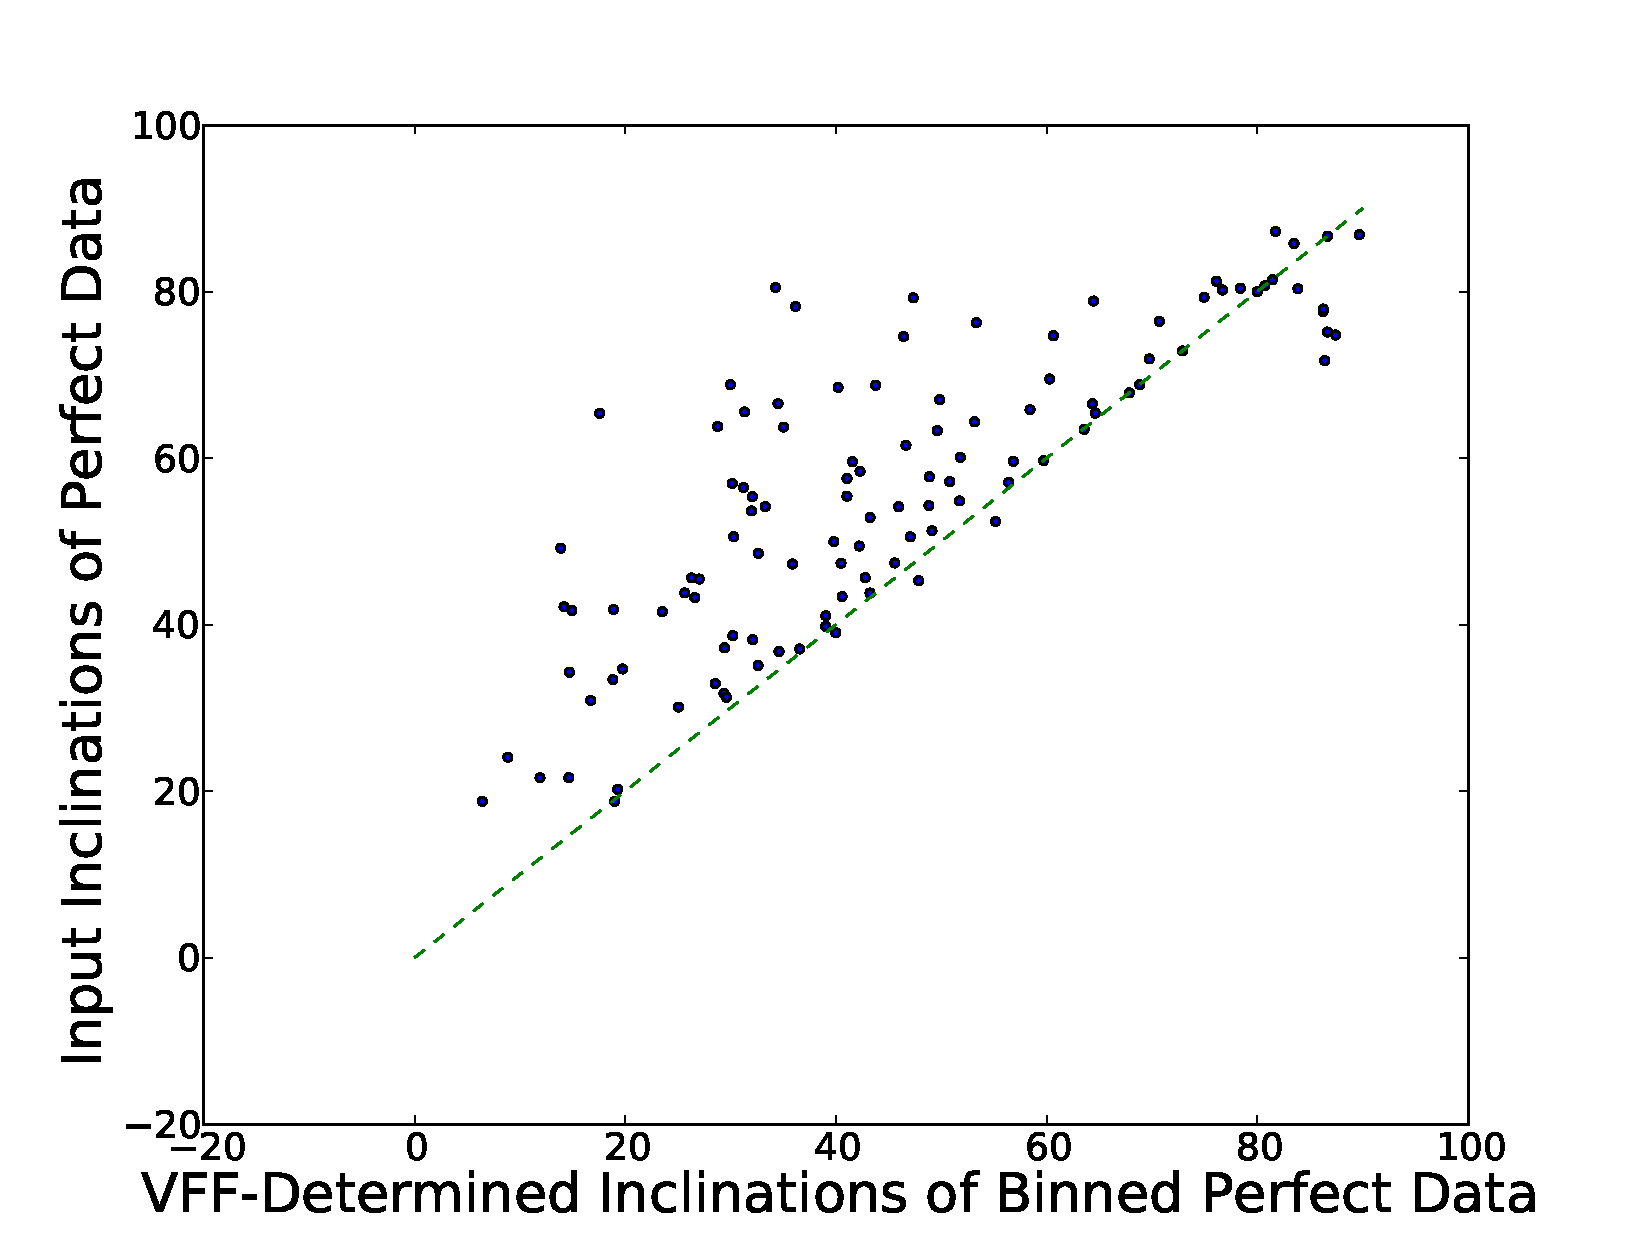
\includegraphics[width=0.5\textwidth]{binnedtest.pdf}
\caption{A comparison of the input inclinations and the inclinations determined from much more poorly sampled perfect velocity fields. \label{fig:test}}
\end{figure}

\subsection{Binned Down Turbulent Fields}
\large This is the ultimate test, and will determine if VFF does okay in the worst case possible, but likely the most realistic. In a future draft of this paper, this test and an analysis will be included.
%%%%%%%% DO THIS TEST AND PLOT THE RESULTS!!!
%%%%%% WRITE FINDINGS FROM CHECKING THIS!!! %%%%%%%%%

\subsection{Real Data}

\begin{figure}[h]
\begin{center}
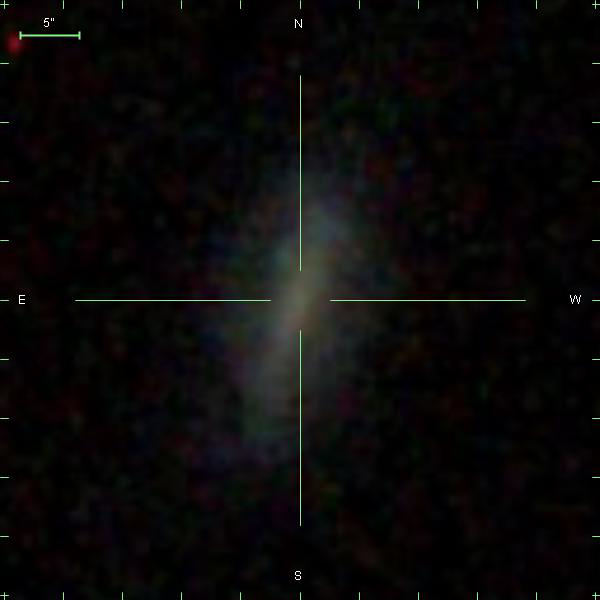
\includegraphics[width=0.34\textwidth]{tinygal.jpg}
\end{center}
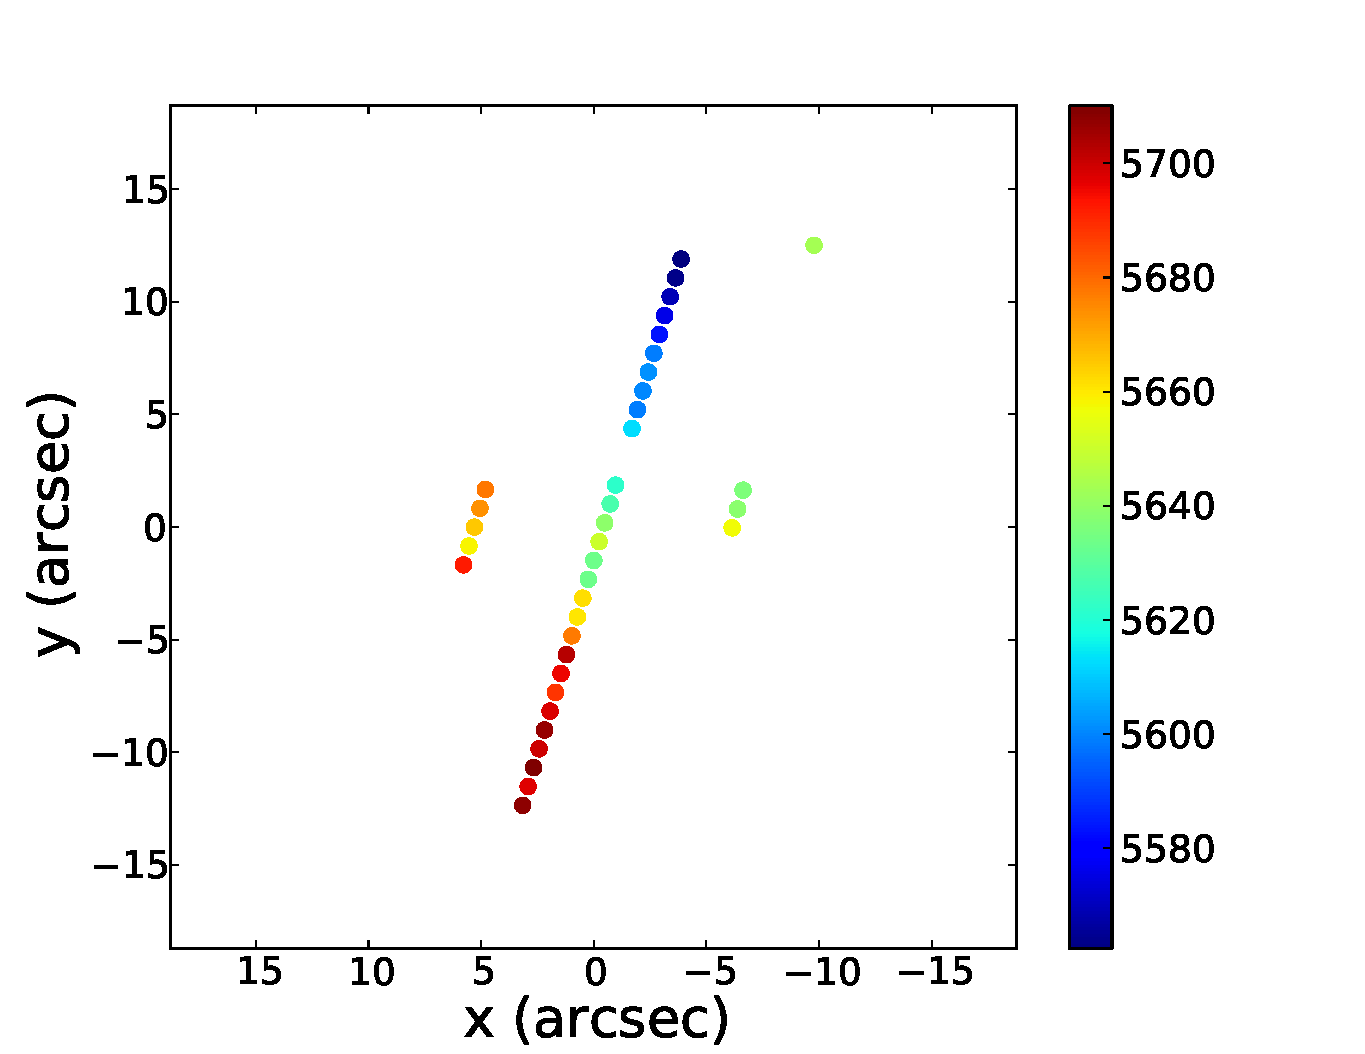
\includegraphics[width=0.5\textwidth]{rawvels.pdf}
\caption{The SDSS image and the SOAR spectrum of a galaxy in the survey. \label{fig:test}}
\end{figure}

\large With real data, VFF fits similarly to DiskFit, but with a larger degree of variance from the photometric counterparts. Further analysis is necessary to describe these effects in detail, but a plot of the galaxy that has been used is shown here along with the data as reduced from the RESOLVE survey.
%%%%%%% PRESENT AN ANALYSIS OF REAL DATA AND PHOTOMETRIC PROPERTIES 
%%%%%%% TO BE DISCUSSED IN DISCUSSIONS AND CONCLUSIONS.


%---------------------------------------------------------------------------------%
%                               Section 5: Discussion                             %
%---------------------------------------------------------------------------------%

\section{Discussion}
\large It would be odd to assume that every spiral galaxy is mostly circular, or even that they all have the same disk height, but we do this frequently in analyses. As one observes more irregular galaxies, it is obvious that the axial ratio of a galaxy is not the only parameter that defines a galaxy's inclination. Since VFF does very well with turbulence, it might be interesting to examine the turbulence found in real samples of data by fitting the velocity field and then subtracting off the fit, as phenomena that cause plane-perpendicular motion such as tidal stripping or merging are phenomena that would assuredly give lower inclination measurements. Is there an easy change that we could make to Hubble's simple equation (1) to give us more accurate results? In the future, we also hope to complete tests of homogeneity of the catalog by looking at the observed and expected distributions of inclinations in the volume.


%%%%%%%% FINISH!!!! %%%%%%%%

\section{Conclusions}
\large We have found that Hubble's photometric inclination measurement technique is not accurate and we have also found that VFF does just as well as DiskFit in most regards but for small galaxies where it significantly outperforms DiskFit, but we have yet to examine the differences between kinematic and photometric inclinations again using VFF, or to compare those differences with photometric properties of galaxies. When this is done, we will be able to answer whether or not there is an easy fix to obtain more accurate photometric inclination measurements, and if so provide a new prescription to accurately defining inclinations of galaxies photometrically. 

\section{Acknowledgements}
\large I would like to first thank Sheila Kannappan for facilitating and consulting on the application of tests in this project. I would like also to thank Charlie Bonfield for his contributions writing the initial code and continuing to aid in the implementation of additional alterations. Finally, I would like to thank team members of the RESOLVE survey for further assistance during the research process. This research was supported in part by the National Science Foundation under an REU supplement to CAREER award AST-0955368.

\bibliographystyle{apj}
\bibliography{references}
%\section{Introduction}
%
%The introduction should contain sufficient
%background on the topic of your research that the reader understands what
%you are doing and why. It is important here and elsewhere in the paper to
%cite references when appropriate. While one can do this manually -- e.g
%(Vollbach et al. 1997), the easiest was to do this is with bibtex and the
%cite commands, because this automatically updates the references in both
%the text and the reference list at the end. For example, you can put the
%reference \cite{hamann2008}, or if you want it in line rather than in
%braces, then \citet{hamann2008}. To compile the documents you must then
%also have a .bib file (e.g. ast4723.bib) that contains the ADS bibtex entry, with
%the article name given as hamann2008, as in the example with this document.
%The document are then compiled by typing:
%
%bibtex ast4723
%latex ast4723.tex ; dvips -o ast4723.ps ast4723.dvi
%latex ast4723.tex ; dvips -o ast4723.ps ast4723.dvi
%
%Mote that you have to latex it twice after adding references for all the references
%to get updated.
%The following examples of sections are intended to provide a rough guideline for how
%you may wish to structure your paper. You are not required to maintain this format,
%but should use a similar, sensible approach.
%
%You may need to have emulateapj.cls in the same directory as your document.
%
%
%\section{Observations}
%
%In this section you should describe your observations. Look at a real paper (or
%at least the sample.tex file with emulateapj) to get an idea for what is appropriate
%in this section. Be sure to include information about what nights you observed
%and any key issues related to your data quality.  If you are using archival data,
%then you should describe when the data was originally obtained and still describe 
%things such as the instrument and telescope.
%
%\section{Data Reductions}
%
%This section is your chance to describe everything that you did to process your data.
%List clearly how you reduced the data and did the photometry. If you wish to divide
%this into subsections, you can do so as illustrated below.
%\subsection{Bias Subtraction and Flatfielding}
%To subtract the bias, we...
%\subsection{Really weird stuff that I had to do for my data}
%There was a bad region shaped like a parrot in the middle of the detector, which required...
%\subsection{Image Stacking}
%We aligned the images using...
%\subsection{Photometric Calibration}
%
%\section{Data Analysis}
%
%This section should describe the scientific analysis done for your project. If you are
%making a light curve for example, here is where you would describe how you made it and what you measured.
%Remember that your write-up should contain figures, such as Figure \ref{fig:test}. Note that this
%reference to the figure is collected to a label in the figure caption, so if you add others the
%number will automatically update
%
%\section{Results and Discussion (can easily be separate sections)}
%
%Fairly self explanatory. You should think carefully about what your results 
%mean. Speculation is good, but it should be grounded in the data -- wild
%speculation is bad.  If you want to add any equations in the text, this
%can be done in the fashion below. Note that the online latex references, 
%including the ones linked off the web page, provide the necessary information
%for constructing more complex equations. If you want to include equation
%symbols inline in the text, then you place them between dollar signs, as
%shown below.
%
%Consider the equation
%\begin{equation}
%\bar v = \exp(\tau^{-1})
%\end{equation}
%where $\bar v$ is the mean velocity of a purple balloon, and $\tau$ is
%the mean free path of the balloon. If we have a velocity $\bar v = 5\pm1$ km s$^{-1}$,
%what is $\tau$?
%
%One last item that we have not discussed is tables. There is an example in this
%document in Table \ref{tab:test}, which is the same as in sample.tex.
%
%\acknowledgments
%
%Anyone whom you would like to thank would go in this section (not required). 
%
%
%\appendix
%
%\section{Appendix material}
%
%If you want to go into a lot of detail about something that you feel doesn't belong
%in the main part of the paper, this would be the place to do it. 
%
%For this document, I will simply note that for the bibliographies, the manual
%way of including a bibliography is
%\begin{verbatim}
%\begin{thebibliography}{}
%\bibitem[Auri\`ere(1982)]{aur82} Auri\`ere, M.  1982, \aap,
%    109, 301
%\bibitem[Canizares et al.(1978)]{can78} Canizares, C. R.,
%    Grindlay, J. E., Hiltner, W. A., Liller, W., \&
%    McClintock, J. E.  1978, \apj, 224, 39
%\bibitem[Djorgovski \& King(1984)]{djo84} Djorgovski, S.,
%    \& King, I. R.  1984, \apjl, 277, L49
%\bibitem[Hagiwara \& Zeppenfeld(1986)]{hag86} Hagiwara, K., \&
%    Zeppenfeld, D.  1986, Nucl.Phys., 274, 1
%\bibitem[Harris \& van den Bergh(1984)]{har84} Harris, W. E.,
%    \& van den Bergh, S.  1984, \aj, 89, 1816
%\bibitem[King(1966)]{kin66}  King, I. R.  1966, \aj, 71, 276
%\bibitem[Ortolani et al.(1985)]{ort85} Ortolani, S., Rosino, L.,
%    \& Sandage, A.  1985, \aj, 90, 473
%\bibitem[Peterson(1976)]{pet76} Peterson, C. J.  1976, \aj, 81, 617
%\end{thebibliography}
%\end{verbatim}
%
%while the automated way, assuming that you have generated a .bib file is

%
%which for the file ast4723.bib and this tex file generates the reference list
%seen below. A nice aspect of this approach is that if you don't use a reference
%in the paper it automatically gets removed from the reference list at the end.
%The one additional file that you need to have for this approach is apj.bst,
%which is posted on the web page.
%
%
%\bibliographystyle{apj}
%\bibliography{references}
%
%\clearpage
%
%\begin{deluxetable}{ccrrrrrrrrcrl}
%\tabletypesize{\scriptsize}
%\tablecaption{Sample table taken from \citet{treu03}\label{tbl-1}}
%\tablewidth{0pt}
%\tablehead{
%\colhead{POS} & \colhead{chip} & \colhead{ID} & \colhead{X} & \colhead{Y} &
%\colhead{RA} & \colhead{DEC} & \colhead{IAU$\pm$ $\delta$ IAU} &
%\colhead{IAP1$\pm$ $\delta$ IAP1} & \colhead{IAP2 $\pm$ $\delta$ IAP2} &
%\colhead{star} & \colhead{E} & \colhead{Comment}
%}
%\startdata
%0 & 2 & 1 & 1370.99 & 57.35    &   6.651120 &  17.131149 & 21.344$\pm$0.006  & 2 4.385$\pm$0.016 & 23.528$\pm$0.013 & 0.0 & 9 & -    \\
%0 & 2 & 2 & 1476.62 & 8.03     &   6.651480 &  17.129572 & 21.641$\pm$0.005  & 2 3.141$\pm$0.007 & 22.007$\pm$0.004 & 0.0 & 9 & -    \\
%0 & 2 & 3 & 1079.62 & 28.92    &   6.652430 &  17.135000 & 23.953$\pm$0.030  & 2 4.890$\pm$0.023 & 24.240$\pm$0.023 & 0.0 & - & -    \\
%0 & 2 & 4 & 114.58  & 21.22    &   6.655560 &  17.148020 & 23.801$\pm$0.025  & 2 5.039$\pm$0.026 & 24.112$\pm$0.021 & 0.0 & - & -    \\
%0 & 2 & 5 & 46.78   & 19.46    &   6.655800 &  17.148932 & 23.012$\pm$0.012  & 2 3.924$\pm$0.012 & 23.282$\pm$0.011 & 0.0 & - & -    \\
%0 & 2 & 6 & 1441.84 & 16.16    &   6.651480 &  17.130072 & 24.393$\pm$0.045  & 2 6.099$\pm$0.062 & 25.119$\pm$0.049 & 0.0 & - & -    \\
%0 & 2 & 7 & 205.43  & 3.96     &   6.655520 &  17.146742 & 24.424$\pm$0.032  & 2 5.028$\pm$0.025 & 24.597$\pm$0.027 & 0.0 & - & -    \\
%0 & 2 & 8 & 1321.63 & 9.76     &   6.651950 &  17.131672 & 22.189$\pm$0.011  & 2 4.743$\pm$0.021 & 23.298$\pm$0.011 & 0.0 & 4 & edge \\
%\enddata 
%%% Text for table notes should follow after the \enddata but before %% the \end{deluxetable}. Make sure there is at least one \tablenotemark
%%% in the table for each \tablenotetext.  
%\tablecomments{Table \ref{tbl-1} is published in its entirety in the electronic edition of the {\it Astrophysical Journal}. A portion is shown here for guidance
%regarding its form and content.}
%
%\tablenotetext{a}{Sample footnote for table~\ref{tbl-1} that was generated
%with the deluxetable environment}
%\tablenotetext{b}{Another sample footnote for table~\ref{tbl-1}}
%
%\end{deluxetable}

\end{document}

%%
%% End of file `sample.tex'.
